\chapter{Introduction}

\label{sec:intro}

The early investigations of elementary particles at the beginning of the 20th century have brought up a radically new theoretical approach, which describes the observed phenomena by gauge symmetry groups. This concept is better known as the Standard Model of elementary particle physics (SM) (see~\cref{sec:SM1}).

The SM has undergone extensive investigations of its properties, which confirm its consistency astonishingly well. Despite the remarkable success of the SM, there are still a lot of open questions. For example astronomical observations  bring up concepts, which are hints that the SM in its present form might not be complete. The constraining of the SM  is a very important task and the investigation of the top-quark might bring up some interesting results in this context. 

The discovery of the top-quark completes the so called quark sector of the SM, which groups one specific particle type. In comparison with the other quarks however, the properties of the top quark are outstanding. A very good example  is its mass $m_{\text{top}}$, which is about forty times larger than the mass of the second heaviest quark, the bottom quark. Furthermore, $m_{\text{top}}$ is a fundamental parameter of the SM, which has a huge impact on certain quantities, like the stability of SM vacuum.  Thus, it is very interesting to investigate this property.

As displayed by~\cref{fig:mass} there have been several measurements of the top-quark mass performed by the CMS and ATLAS collaboration~\cite{PubR}. The shown results belong to different decay channels. Furthermore, the current world average value of 173.55 $\pm$ 0.5~GeV is displayed (orange)~\cite{ATLAS:2014wva}, which also takes the results from the Tevatron measurements into account. Several measurements (green) have been performed by the ATLAS group of the Max-Planck-Institute for Physics in Munich (MPP). The results stem from the so-called dileptonic decay channel and the lepton + jets decay channel. At the MPP, the measurements of the top-quark mass in both channels were performed for a center-of-mass energy of 7 and 8~TeV~\cite{Aad:2015nba,Aaboud:2016igd,ATLAS-CONF-2017-071}. 
The latest combination of the two decay channels  (for the  8~TeV results) gives a top-quark mass value of 172.51 $\pm$ 0.5~GeV (grey)~\cite{ATLAS-CONF-2017-071}.





For this analysis, the $t\bar{t}\rightarrow$lepton + jets channel is used. 
In events of this kind, a top-antitop quark pair is produced. One of the quarks decays into a lepton pair, and a so-called $b$ quark, while the second one decays into a  $b$ quark  and additional light quarks. The $b$ quarks and the light quarks trigger  particle showers, which can be identified with the experiment as hadronic particle showers, the so called jets). 
The basic idea of this thesis is to perform the  
$m_{	\rm top}$ measurement, in the same way as it was done in the previous analyses~\cite{Aad:2015nba,ATLAS-CONF-2017-071}, using the so-called template method, which is based on simulated distributions of observables, which are sensitive to the top-quark mass.  

As shown by the previous analyses, there are large uncertainties affecting the top-quark mass measurement, arising from the so-called jet energy scales JES and bJES (see~\cref{JES}). This energy scales are related to the calibration of the measured particle showers. Therefore, a three dimensional  approach of the template method is performed, which determines the top-quark mass together with the  so called jet energy scale factors JSF and bJSF. The introduction of the two jet scale factors provide the sensitivity to the jet energy scales, which  allows mitigating the corresponding
systematic uncertainties on the top-quark mass and  to absorb the uncertainties arising from the jet energies, using the  multidimensionality of the fit. 
For the simultaneous measurement of the top-quark mass and the two scale factors,  Monte Carlo simulated distributions of chosen observables are used as estimators. These distributions are obtained from the event kinematics of the lepton + jets decay (see~\cref{ch5}).  
 From the simulated templates, probability distributions are obtained, in order to perform an unbinned  maximum likelihood fit to determine the top-quark mass.
  A detailed introduction and motivation of the three dimensional template method is given in~\cref{sec:Temp1}.

The main task of this master project has been the implementation of the analysis workflow in new framework and perfrome the measurement to the new 13~TeV data and simulation, while  following the analysis steps of the previous analyses.  Nevertheless, with respect to the official ATLAS analysis, which is currently work in progress, the final likelihood fit is here not performed to the data and therefore, there is no specific value of for the top-quark mass. One should instead consider this thesis as preparation and test for the final ATLAS analysis with the framework applied to the  new data  and simulation.

This thesis is structured like the analysis workflow. After a short introduction of the Standard Modell of particle physics and the top-quark, the ATLAS experiment is briefly described. In the next chapters, the physical objects, which are used in this analysis are introduced as well as the first analysis step, the event selection. In~\cref{ch5} the event reconstruction is described, which is used to construct the three estimator distributions for the measurement of the top-quark and the scale factors. The final extraction with the template method is motivated in~\cref{sec:Temp1}. Finally the evaluation of the systematic uncertainties is given (see~\cref{sec:Uns}), followed by a short summery in~\cref{sec:sum}.




\begin{figure}[h]
	\centering
	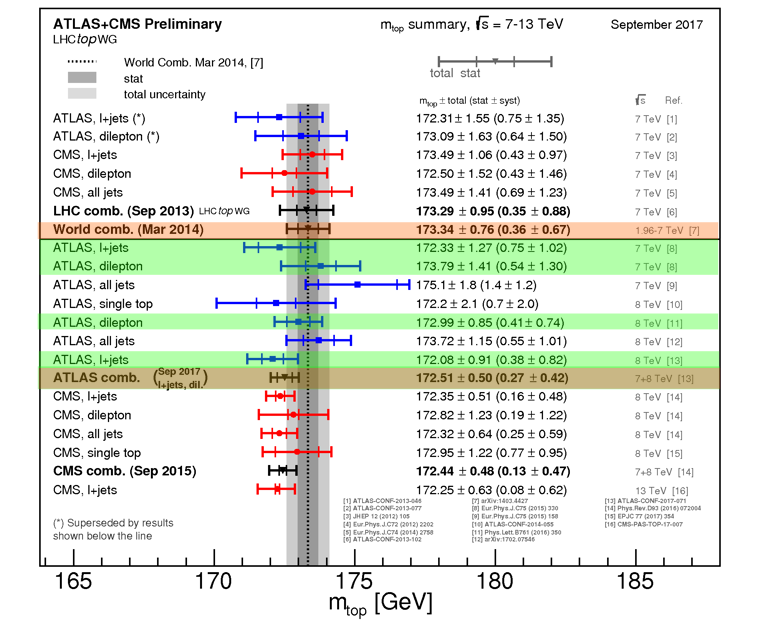
\includegraphics[width=0.8\linewidth]{Pics/mass}
	\caption{Summary of top-quark mass measurements, performed by the CMS and the ATLAS collaboration~\cite{PubR}. }
	
	\label{fig:mass}
\end{figure}



